\documentclass[11pt]{article}
\setlength{\topmargin}{-.5in}
\setlength{\textheight}{9in}
\setlength{\oddsidemargin}{.125in}
\setlength{\textwidth}{6.25in}

\usepackage{graphicx}
\usepackage{amsmath}
\usepackage{amsthm}
\usepackage{proof}
\usepackage{algorithm}
\usepackage{algorithmic}
\usepackage{dsfont}
\usepackage{parsetree}

\usepackage{float} % for box around all figures
\floatstyle{boxed} 
\restylefloat{figure}

\begin{document}

\title{Stochastic linear indexed grammars for simple repeat recognition in biological data}

\author{M.L. Souza\\
University of California Berkeley\\
Biophysics}

\renewcommand{\today}{June 13, 2011}
\maketitle
This article explores the use and limitations of stochastic linear indexed grammars for recognition of mobile element-like sequences.

\section {Motivation}
Context-free grammars (CFGs) are well suited to modeling of arbitrarily complex nestings of dyad symmetry in sequences.
However, CFGs are incapable of generating languages of direct repeats; and thus biological languages are frequently beyond context-free.
Here we consider the application of extensions to CFGs capable of limited generation of repeats, while preserving
polynomial parsing complexity. \\ \\
In the following, we consider a few motivating examples of repetition in transposon sequences. Let $T^*$ be the Kleene closure of a set of terminal symbols, e.g. $T = \left \{ A,C,G,T \right \}$,
and let $\overline{w}^R$ denote the ``inverted repeat'' of $w$. (E.g. for $w = CTGGA$, $\overline{w}^R = TCCAG$.)

\subsection {Repeats Flanking Inverted Repeats}
Class II DNA transposons have sequence structure consisting of a variable region surrounded by inverted repeats.
Such inverted repeats are precisely the dyad structure that CFGs are suited for.\\
However, flanking the inverted repeats there exist short direct repeats from the process of transposition.
The class of languages resembles the following:
\[
L_{SRIR} = \left \{ y(wx\overline{w}^R)y \mid w,\overline{w}^R,x,y \in T^* \right \} 
\]

\subsection {LTR Retrotransposons}
Class I retrotransposons have a structure as shown in figure \ref{fig:LTR}. Their distinctive structural feature is precisely
what makes them unsuited for recognition by CFGs; flanking terminal repeats.
\begin{figure}[H] 
  \centering 
  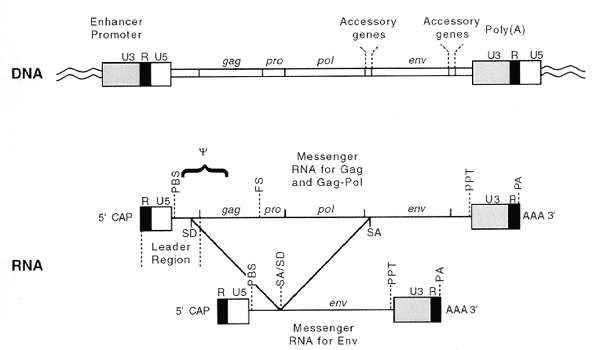
\includegraphics[scale=0.5]{./figure2-4.jpg}
  \caption{(Figure stolen from: \cite{CoffinJMHughesSHVarmusHE1997} Fix me.)}
  \label{fig:LTR}
\end{figure}
This class of languages is:
\[
\L_{LTR} = \left \{ wxw \mid w,x \in T^* \right \}
\]

\subsection {Insertion Sequences}
The form of an insertion sequence has both dyad symmetry and a direct repeat structure, separated by sequences coding
for transposition and structural machinery.
\begin{figure}[H]
  \centering 
  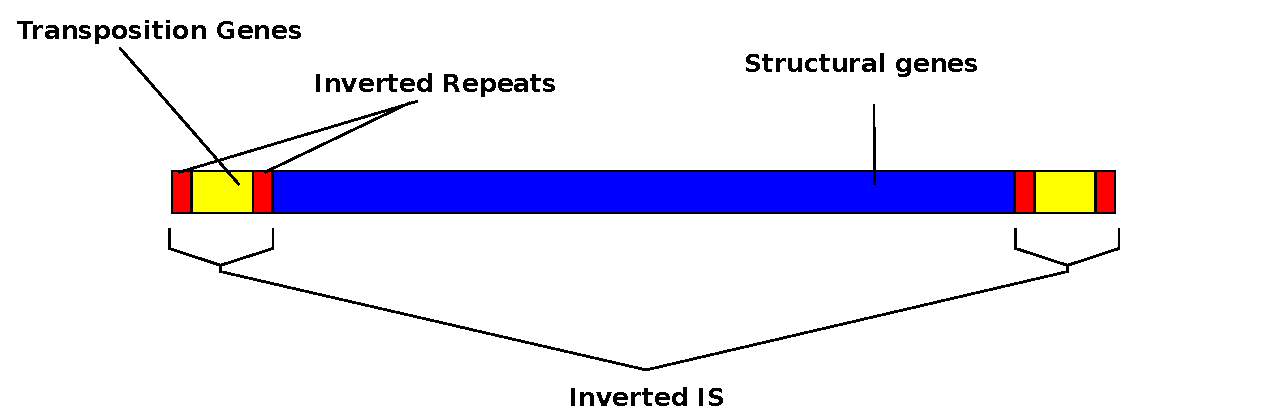
\includegraphics[scale=0.50]{./Composite_transposon.pdf}
  \caption{(Figure stolen and modified from wikipedia transposable element page. Fix me.)}
  \label{fig:IS}
\end{figure}
\noindent
The class of languages describing insertion sequences is roughly:\\
\[
\L_{IS} = \left \{ (wx\overline{w}^R)y(wx\overline{w}^R) \mid w,\overline{w}^R,x,y \in T^* \right \}
\]
Note that this language is a more structured form of $\mathds{L}_{LTR}$.\\
\section {Extended Context-Free Grammars}
In this section we introduce indexed grammars.
\subsection {Review of CFGs}
Context-free grammars are defined as a 4-tuple: $G = (N, T, P, S)$ where $N$ is a set of non-terminals; $T$ is a set of terminals; $P$ is a set of production (rewrite) rules;
and $S$ a designated start symbol.\\
Each production rule maps a single non-terminal symbol to any combination of terminal and non-terminal that is substituted in the LHS non-terminal's place in a derivation.\\
An example CFG generating perfect inverted repeats in DNA has production rules:
\[
 S \rightarrow aSt \ | \ tSa \ | \ cSg \ | \ gSc \ | \ \epsilon
\]
An example derivation using the above grammar:\\
\[
 S \Rightarrow cSg \Rightarrow ctSag \Rightarrow  ctgScag \Rightarrow  ctggSccag \Rightarrow  ctggaStccag \Rightarrow  ctggatccag
\]
The above example intuitively demonstrates how CFGs are suited to generate nestings of correlated symbols.
The process of recognition by a CFG's analogous pushdown automaton provides another interpretation.
The symbols of the pushdown stack can only be emitted in a last-in-first-out way; the ``memory'' of
the already-emitted sequence only plays in reverse like a ball rolling back down a hill, producing dyad symmetry.
Thus it's the memory accession method for CFGs that results in their being unsuited to direct repetition. \\ \\
The inability of a CFG to produce a language of repeats can also be shown formally using the Pumping Lemma, which we demonstrate later.
\subsection {Indexed Grammars}
The Indexed Grammars are context-free grammars extended with stacks of indices associated with each non-terminal.
\subsubsection {Definition}
Let $G \ = \ (N, T, I, S, P)$ where $N$ is a set of non-terminals; $T$ a set of terminals, $I$ a set of index symbols,
$S \in N$ a start symbol, and $P$ the set of production rules.
Let $A, B, C \in N$ be non-terminal symbols, $\alpha \in (T \cup N)^*$ be a string of terminals/nonterminals, 
and $i_1, i_2, i_3 \in I$ be index symbols, and $\sigma, \sigma_1, \sigma_2 \in I^*$ be arbitrary (possibly empty) strings of index symbols. \\ \\
Each non-terminal in a production rule in a string such as $\alpha$ has an independent stack of symbols which can optionally inherit and modify the stack passed on the LHS non-terminal.\\
We demonstrate stack passage and modification in IG rewrite rules by example:
\begin{enumerate}
\item $\ \ A[\sigma] \rightarrow A[\sigma]A[\sigma \ i_1 \ i_2]B$ \\ Has stack $[\sigma]$ is passed to the left-most $A$, $[\sigma]$ passed and extended with symbols $i_1, i_2$ to the middle $A$, and the stack of $B$ unmodified.
\item $\ \ A[\sigma \ i_1 \ i_2 \ i_3] \rightarrow B[\sigma]$ \\ Has $i_1, i_2, i_3$ removed from $A$'s stack, and the remainder passed to $B$.
\end{enumerate}
\subsubsection{Example: $L_{IS}$}
Consider the grammar $G_{IS} = (N, T, I, S, P)$ defined as follows:
$T = \left\{a,c,g,t\right\}$, $N = \left\{C, \ X, \ Y, \ R_1 \ R_2 \ R_3\right\}$, $I = \left\{C_{a}, \ C_{g}, \ C_{c}, \ C_{t}, \ X_{a}, \ X_{g}, \ X_{c}, \ X_{t}\right\}$,
$S = C$. \\ \\
Define P with the following rules:\\
\begin{enumerate}
\item $\ \ C[\sigma] \rightarrow a C[\sigma \ C_a] \ | \ g C[\sigma \ C_g] \ | \ c C[\sigma \ C_c] \ | \ t \ C[\sigma \ C_t] \ | \ X[\sigma]$
\item $\ \ X[\sigma] \rightarrow a X[\sigma \ X_a] \ | \ g X[\sigma \ X_g] \ | \ c X[\sigma \ X_c] \ | \ t \ X[\sigma \ i_t] \ | \ R_1[\sigma] \ Y[] \ R_2[\sigma] \ R_1[\sigma]$
\item $\ \ Y[\sigma] \rightarrow a Y[\sigma] \ | \ g Y[\sigma] \ | \ c Y[\sigma] \ | \ t Y[\sigma] \ | \ \epsilon$
\item $\ \ R_1[\sigma \ C_a] \rightarrow t R_1[\sigma], \ R_1[\sigma \ C_g] \rightarrow c R_1[\sigma], \ R_1[\sigma \ C_c] \rightarrow g R_1[\sigma], \ R_1[\sigma \ C_t] \rightarrow a R_1[\sigma]$
\item $\ \ R_1[\sigma \ X_a] \rightarrow R_1[\sigma], \ R_1[\sigma \ X_g] \rightarrow R_1[\sigma], \ R_1[\sigma \ X_c] \rightarrow R_1[\sigma], \ R_1[\sigma \ X_t] \rightarrow R_1[\sigma]$
\item $\ \ R_1[] \rightarrow \epsilon$, $\ R_2[] \rightarrow \epsilon$
\item $\ \ R_2[\sigma \ C_a] \rightarrow R_2[\sigma] a, \ R_2[\sigma \ C_g] \rightarrow R_2[\sigma] g, \ R_2[\sigma \ C_c] \rightarrow R_2[\sigma] c, \ R_2[\sigma \ C_t] \rightarrow R_2[\sigma] t$
\item $\ \ R_2[\sigma \ X_a] \rightarrow R_2[\sigma] a, \ R_2[\sigma \ X_g] \rightarrow R_2[\sigma] g, \ R_2[\sigma \ X_c] \rightarrow R_2[\sigma] c, \ R_2[\sigma \ X_t] \rightarrow R_2[\sigma] t$
\end{enumerate}
This grammar generates $\mathds{L}_{IS}$. \\
For example, the following is a derivation of the sequence ACG \ T \ CGT \ A \ ACG \ T \ CGT: \\
\indent$ C \ \overset{1.1}{\Rightarrow} a C[C_a] \overset{1.3}{\Rightarrow} ac C[C_a, C_c] \overset{1.2}{\Rightarrow} acg C[C_a, C_c, C_g] $ \\
\indent\indent$            \overset{1.5}{\Rightarrow} acg \ X[C_a, C_c, C_g] \overset{2.4}{\Rightarrow} acgt X[C_a, C_c, C_g, X_t] $ \\
\indent\indent$            \overset{2.5}{\Rightarrow} acgt \ R_1[C_a, C_c, C_g, X_t] \ Y[] \ R_2[C_a, C_c, C_g, X_t] \ R_1[C_a, C_c, C_g, X_t] $ \\
\indent\indent$            \overset{3.1}{\Rightarrow} acgt \ R_1[C_a, C_c, C_g, X_t] \ aY[] \ R_2[C_a, C_c, C_g, X_t] \ R_1[C_a, C_c, C_g, X_t] $ \\
\indent\indent$            \overset{3.5}{\Rightarrow} acgt \ R_1[C_a, C_c, C_g, X_t] \ a \ R_2[C_a, C_c, C_g, X_t] \ R_1[C_a, C_c, C_g, X_t] $ \\
\indent\indent$            \overset{5.4 \ x2}{\Rightarrow} acgt \ R_1[C_a, C_c, C_g] \ a \ R_2[C_a, C_c, C_g, X_t] \ R_1[C_a, C_c, C_g] $ \\
\indent\indent$            \overset{4.2 \ x2}{\Rightarrow} acgt \ c \ R_1[C_a, C_c] \ a \ R_2[C_a, C_c, C_g, X_t] \ cR_1[C_a, C_c] $ \\
\indent\indent$            \overset{4.3 \ x2}{\Rightarrow} acgt \ cg \ R_1[C_a] \ a \ R_2[C_a, C_c, C_g, X_t] \ cg R_1[C_a] $ \\
\indent\indent$            \overset{4.1 \ x2}{\Rightarrow} acgt \ cgt \ R_1[] \ a \ R_2[C_a, C_c, C_g, X_t] \ cgt R_1[] $ \\
\indent\indent$            \overset{6.1 \ x2}{\Rightarrow} acgtcgta \ R_2[C_a, C_c, C_g, X_t] \ cgt $ \\
\indent\indent$            \overset{8.4}{\Rightarrow} acgtcgta \ R_2[C_a, C_c, C_g] \ t \ cgt $ \\
\indent\indent$            \overset{7.2}{\Rightarrow} acgtcgta \ R_2[C_a, C_c] \ g \ t cgt $ \\
\indent\indent$            \overset{7.3}{\Rightarrow} acgtcgta \ R_2[C_a] \ cg \ t cgt $ \\
\indent\indent$            \overset{7.1}{\Rightarrow} acgtcgta \ R_2[] \ acg \ t cgt $ \\
\indent\indent$            \overset{6.2}{\Rightarrow} acgtcgtaacgtcgt $ \\

The indexed languages are a proper subset of context-sensitive languages, but the general recognition problem for the indexed grammars is NP-complete. 
Several forms of indexed grammars exist which maintain parsing efficiency by restricting the way in which the stack can be inherited.\\

\subsection {Linear Indexed Grammars}
\subsubsection {Definition}
In {\bf linear indexed grammars} (LIGs) [(defined in 1988 by Gazdar; can't find a copy of the PDF. Fix me.), only one non-terminal can inherit the stack in a rewrite rule.\\ \\
Let $\left \{ w_1, w_2, ..., w_{n+1} \right \} \in T^*$, $\left \{ A_1, \cdots, A_n, A \right \} \in N$, and $\left \{\alpha_1, \alpha_2, \cdots, \alpha_n \right \} \in I^*$ \\
The general form for LIG rewrite rules is:\\
\[
A[\sigma] \rightarrow w_1 A_1[\alpha_1] w_2 A_1[\alpha_2] \cdots w_i A_i[\cdot \cdot \alpha_i] \cdots w_n A_n[\alpha_n] w_{n+1}
\]
\ \\
The non-terminal $A_i[\cdot \cdot \alpha_i]$ in the above rule is the one that inherits the stack, and is known as the {\bf distinguished child of $A[\cdot \cdot \alpha]$}.
In this document when the distinguished child non-terminal is apparent we omit the ``$\cdot \cdot$'' in denoting the stack $[\cdot \cdot \sigma]$.
\subsubsection {Examples}
Note that in the above example of an indexed grammar for $L_{IS}$, rule 2.5 violates the LIG requirement since the stack is inherited by three non-terminals.
We later consider whether LIGs can produce this language.\\ \\
{\bf Consider the language $L_{LTR}$.}\\
This language is considerably less structured than $L_{IS}$, and can be generated with the following grammar $G_{LTR} 
 = (N, T, I, S, P)$ defined as follows: \\ \\
$T = \left\{a,c,g,t\right\}$, $N = \left\{C, \ X, \ C_R\right\}$, $I = \left\{a, \ g, \ c, \ t\right\}$,
$S = C$. \\
Define P with the following rules:
\begin{enumerate}
\item $\ \ C[\sigma] \rightarrow a C[\sigma \ C_a] \ | \ g C[\sigma \ C_g] \ | \ c C[\sigma \ C_c] \ | \ t \ C[\sigma \ C_t] \ | \ X[\sigma]$
\item $\ \ X[\sigma] \rightarrow a X[\sigma] \ | \ g X[\sigma] \ | \ c X[\sigma] \ | \ t \ X[\sigma] | C_R[\sigma]$
\item $\ \ C_R[\sigma \ a] \rightarrow C_R[\sigma] a, \ C_R[\sigma \ g] \rightarrow C_R[\sigma] g, \ C_R[\sigma \ c] \rightarrow C_R[\sigma] c, \ C_R[\sigma \ t] \rightarrow C_R[\sigma] t$
\item $\ \ C_R[] \rightarrow \epsilon$
\end{enumerate}
The sequence $ACGT \ TC \ ACGT$ can be derived as follows:\\
\indent$ C \ \overset{1.1}{\Rightarrow} a C[a] \overset{1.3}{\Rightarrow} ac C[a, c] \overset{1.2}{\Rightarrow} acg C[a, c, g] \overset{1.2}{\Rightarrow} acgt C[a, c, g, t] $ \\
\indent\indent$            \overset{1.5}{\Rightarrow} acgt \ X[a, c, g, t]$ \\
\indent\indent$            \overset{2.3}{\Rightarrow} acgt \ \overset{1.4}{\Rightarrow} acgt \ t X[a, c, g, t] \ \overset{1.3}{\Rightarrow} acgt \ tc X[a, c, g, t] \ \overset{1.5}{\Rightarrow} acgt \ tc C_R[a, c, g, t]$ \\
\indent\indent$            \overset{3.4}{\Rightarrow} acgttc \ C_R[a, c, g] \ t \ \overset{3.2}{\Rightarrow} acgttc \ C_R[a, c] \ gt \ \overset{3.3}{\Rightarrow} acgttc \ C_R[a] \ cgt \overset{3.1}{\Rightarrow} acgttc \ C_R[] \ acgt$ \\
\indent\indent$            \overset{4.1}{\Rightarrow} acgttcacgt$ \\ \\ \\
{\bf Next, we consider the language $L_{SRIR}$.} \\
Consider the grammar $G_{SRIR} = (N, T, I, S, P)$ defined as follows:\\ \\
$T = \left\{a,c,g,t\right\}$, $N = \left\{Y, \ X, W, \ Y_R\right\}$, $I = \left\{a, \ g, \ c, \ t\right\}$,
$S = Y$. \\
Define P with the following rules:
\begin{enumerate}
\item $\ \ Y[\sigma] \rightarrow a Y[\sigma \ a] \ | \ g Y[\sigma \ g] \ | \ c Y[\sigma \ c] \ | \ t \ Y[\sigma \ t] \ | \ C \ Y_R[\sigma]$
\item $\ \ C[] \rightarrow a C[\sigma] t \ | \ t C[\sigma] a \ | \ c C[\sigma] g \ | \ g C[\sigma] c \ | \ X[\sigma]$
\item $\ \ X[] \rightarrow a X[\sigma] \ | \ g X[\sigma] \ | \ c X[\sigma] \ | \ t \ X[\sigma] \ | \ \epsilon$
\item $\ \ Y_R[\sigma \ a] \rightarrow Y_R[\sigma] a, \ Y_R[\sigma \ g] \rightarrow Y_R[\sigma] g, \ Y_R[\sigma \ c] \rightarrow Y_R[\sigma] c, \ Y_R[\sigma \ t] \rightarrow Y_R[\sigma] t$
\item $\ \ Y_R[] \rightarrow \epsilon$
\end{enumerate}
and consider the derivation of $AA \ CGAC \ T \ GTCG \ AA$:
(Fix me.)
\subsection{Going Probabilistic}
Strict duplication as we generate in $G_{IS}$, and $G_{LTR}$ is insufficient to describe real data
due to the imperfection of repetition seen in nature. Such ``imperfection'' sometimes isn't just tolerated error, but is essential for biological activity. \cite{Strawbridge2010} \cite{Costello1995} \\ \\
To address this, we construct grammars with patterns accommodating the exceptions but we adjust for indiscriminate false-positives
by associating probabilities with emissions. \\ \\
We assign probabilities (weights) to each production rule of the grammar such that the
sum of the weights of all productions from any single non-terminal is 1,\\
i.e. $\displaystyle\sum\limits_{\alpha}^{} P(X \rightarrow \alpha) = 1$ for all rules ($X \rightarrow \alpha$) $\in P$. \\ \\
The grammar $G$ produces a probability distribution over its emitted strings $s$: $\displaystyle\sum\limits_{s}^{} P(s \ | \ G) = 1$.\\ \\
We're interested in ways to address the following problems:
\begin {enumerate}
 \item {\bf Scoring}: Calculate $P(s \in T^* \ | \ G)$ \\
  Given a stochastic grammar, calculate the probability of it having emitted a sentence.
 \item {\bf Training}: $W$ s.t. $E\left[P(t_1, t_2, \cdots, t_m \ | \ G)\right]$ is maximal. \\
  (Exposition here about how probabilities are defined/refined)
  Given a set of positive-matching examples, we want to re-estimate the production weight distribution 
  such that the probabilities of emitting the example sequence are maximized.
\end {enumerate}
Below we consider how LIGs are extended to become probabilistic. Later in the section on parsing, we consider methods to address the above two problems.
\subsubsection {Stochastic LIGs}
We define a stochastic LIG (SLIG) by a 6-tuple: $G \ = \ (N, T, I, S, P, W)$ where $N$ is a set of non-terminals; $T$ a set of terminals, $I$ a set of index symbols,
$S \in N$ a start symbol, $P$ the set of production rules, and $W \ : \ P \rightarrow \mathds{R}$ is a rule weight function. \\ \\
In defining $W$ over the set of productions, we incorporate the stack into the probability definition with: $\displaystyle\sum\limits_{\alpha}^{} P(X[\cdot \cdot i] \rightarrow \alpha) = 1$ for all rules ($X[\cdot \cdot i] \rightarrow \alpha$) $\in P$. \\ \\
\ \\
As an example, we modify the grammar $G_{LTR}$ above to generate imperfect repeats:\\
Consider the grammar $SG_{LTR} = (N, T, I, S, P, W)$ defined as follows: \\ \\
$T = \left\{a,c,g,t\right\}$, $N = \left\{C, \ X, \ C_R\right\}$, $I = \left\{a, \ g, \ c, \ t\right\}$,
$S = C$. \\
Define $P, W$ with the following rules: (W defined by listing rule probabilities to the right)
\begin{enumerate}
\item 
  \begin{enumerate}
    \item $C[\sigma] \ \rightarrow \ a C[\sigma \ C_a]$ {\bf 0.2075}
    \item $C[\sigma] \ \rightarrow \ a C[\sigma \ C_g]$ {\bf 0.01}
    \item $C[\sigma] \ \rightarrow \ a C[\sigma \ C_c]$ {\bf 0.01}
    \item $C[\sigma] \ \rightarrow \ a C[\sigma \ C_t]$ {\bf 0.01}
    \item $C[\sigma] \ \rightarrow \ g C[\sigma \ C_a]$ {\bf 0.01}
    \item $C[\sigma] \ \rightarrow \ g C[\sigma \ C_g]$ {\bf 0.2075}
    \item $C[\sigma] \ \rightarrow \ g C[\sigma \ C_c]$ {\bf 0.01}
    \item $C[\sigma] \ \rightarrow \ g C[\sigma \ C_t]$ {\bf 0.01}
    \item $C[\sigma] \ \rightarrow \ c C[\sigma \ C_a]$ {\bf 0.01}
    \item $C[\sigma] \ \rightarrow \ c C[\sigma \ C_g]$ {\bf 0.01}
    \item $C[\sigma] \ \rightarrow \ c C[\sigma \ C_c]$ {\bf 0.2075}
    \item $C[\sigma] \ \rightarrow \ c C[\sigma \ C_t]$ {\bf 0.01}
    \item $C[\sigma] \ \rightarrow \ t C[\sigma \ C_a]$ {\bf 0.01}
    \item $C[\sigma] \ \rightarrow \ t C[\sigma \ C_g]$ {\bf 0.01}
    \item $C[\sigma] \ \rightarrow \ t C[\sigma \ C_c]$ {\bf 0.01}
    \item $C[\sigma] \ \rightarrow \ t C[\sigma \ C_t]$ {\bf 0.2075}
    \item $C[\sigma] \ \rightarrow \ X[\sigma]$ {\bf 0.05}
  \end{enumerate}
\item
  \begin{enumerate}
    \item $X[\sigma] \ \rightarrow \ a X[\sigma]$ {\bf 0.2375}
    \item $X[\sigma] \ \rightarrow \ g X[\sigma]$ {\bf 0.2375}
    \item $X[\sigma] \ \rightarrow \ c X[\sigma]$ {\bf 0.2375}
    \item $X[\sigma] \ \rightarrow \ t X[\sigma]$ {\bf 0.2375}
    \item $X[\sigma] \ \rightarrow \ C_R[\sigma]$ {\bf 0.05}
  \end{enumerate}
\item
  \begin{enumerate}
    \item $C_R[\sigma \ a] \ \rightarrow \ C_R[\sigma] a$ {\bf 1.0}
    \item $C_R[\sigma \ g] \ \rightarrow \ C_R[\sigma] g$ {\bf 1.0}
    \item $C_R[\sigma \ c] \ \rightarrow \ C_R[\sigma] c$ {\bf 1.0}
    \item $C_R[\sigma \ t] \ \rightarrow \ C_R[\sigma] t$ {\bf 1.0}
    \item $C_R[] \ \rightarrow \ \epsilon$ {\bf 1.0}
  \end{enumerate}
\end{enumerate}
In rule $1.a$ to $1.l$ above, the majority of weight is given to canonical base-pairing, and low (1\%) probability to non-canonical pairings.
Also note in rule $3.a$ to $3.e$ how each emission has unit mass due to the association of the matching index with the non-terminal; in a SCFG,
the mass would be distributed amongst each of the 5 rules having non-terminal $C_R$ on the LHS.\\ \\
We discuss the methods for calculating probabilities of interest below in the parsing section. (PUT A BETTER INTERNAL REFERENCE HERE. Fix me.) \\

\subsection {Equivalent Formalisms}
\subsubsection {Tree Substitution Grammars}
We first consider the formalism of {\bf Tree Substitution Grammars} (TSGs).\\ \\
Tree substitution grammars allow for the explicit statement of the structure of parse trees which context-free grammars ultimately produce.
But unlike the rule rewriting of a CFG, the elementary operation is the substitution of one elementary sub-tree of a parse into another at 
designated locations.\\
In this way, explicit relationships can be modeled without having to resort to specialized constraints within rule rewriting. \\ \\
For instance in the following TSG:\\ 
\begin{parsetree}
    ( .$NT_0$. 
        `${\bf NT_1} \downarrow$'
        ( .$NT_2$.
            (.$NT_3$.    `${\bf NT_6} \downarrow$' )
            (.$NT_4$.    `$T_2$' )
            (.$NT_5$.    `$T_3$' )
         )
    )
\end{parsetree}
\begin{parsetree}
    ( .$NT_1$. 
        `$FIRSTT_1$'
    )
\end{parsetree}
\begin{parsetree}
    ( .$NT_1$. 
        `$FIRSTT_2$'
    )
\end{parsetree}
\begin{parsetree}
    ( .$NT_6$. 
        `$SECONDT_1$'
    )
\end{parsetree}
\begin{parsetree}
    ( .$NT_6$. 
        `$SECONDT_2$'
    )
\end{parsetree}\\ \\
%The sequences: ${FIRSTT_1}.{SECONDT_1}.{T_2}.{T_3}$, ${FIRSTT_2}.{SECONDT_1}.{T_2}.{T_3}$, e.t.c. can be generated
%very easily, where as imposing the constraint that the terminal symbols $FIRSTT_i$, and $FIRSTT_j$ in a CFG becomes more troublesome.
%This ease of specification is known as the domain of locality. \ref{addreftotreeadjoininggrammarsbyabeillehere} \\ \\
Tree substitution grammars and CFGs have the same weak generative capacity, thus they're not ``extensions'' of CFGs.
However in their weak equivalence to CFGs they serve as a stepping stone to understanding how the next class of grammars is an extension of generative capacity.

\subsubsection {Tree Adjoining Grammars}
If we begin with a TSG, and add the ability to embed one elementary tree within another (in a process known as ``adjoining'') then we
arrive at the formalism of {\bf Tree Adjoining Grammars}.\\
Write about weak/strong generative capacity equivalence to LIGs.\\
Write about going from TAG <-> LIG.\\
%More specifically, in the TAG formalism we consider two classes of ``elementary trees'', \\
Fix me.

\subsubsection {The Other Formalisms}
Fix me.

\section {The Limitations of Grammars}
We now consider the inherent limitations the formalism we adopt imposes on the complexity of the sequences we can match.
\subsection {Pumping Lemmas}
In section 2.1, the inability of CFGs to generate a language of copies was intuitively discussed.
The {\bf pumping lemmas} provide tools with which we can prove this and similar claims more rigorously.
They are a collection of theorems that give necessary (but not sufficient) conditions that languages must satisfy to exist within
a given class. In practice they can provide a way to show when a grammar {\bf can't} generate a language.

\subsubsection {Pumping Lemma for Regular Grammars}
As the complexity of the formalism increases so does the pumping argument machinery, and so
for the sake of pedagogy, we begin with regular grammars and their inability to produce a characteristically
context-free language: palindromes.

\subsubsection {Pumping Lemma for CFGs}
The Pumping Lemma for Context-Free Languages is as follows:
\newtheorem{thm:bar-hillel}{Bar-Hillel Theorem}
\begin{thm:bar-hillel} \label{thm:bar-hillel}
\begin{algorithmic}
\ \\
\IF {$\left ( \mathds{L} \ is \ {Context \ Free} \right )$}
  \STATE $Pumping \ property \ must \ hold:$
  \STATE $\exists \ p \in \mathds{Z} \ s.t.$
  \STATE $\ \ \forall s \in \mathds{L} \left (with \ \left | s \right | \geq \ p, \ s = uvxyz, \ \left | vxy \right | \leq \ p, \ \& \ \left | vy \right | \geq 1 \right ): $
  \STATE $\ \  \ \ \ \ \ \ \ \ \forall n \in \mathds{N} \cup \left \{ 0 \right \}, u(v^n)x(y^n)z \in \mathds{L}$
\ENDIF
\end{algorithmic}
\end{thm:bar-hillel}

\ \\
We can use this theorem to show that no CFG can produce language $L_{LTR}$:\\
\begin{proof}
Suppose thm. \ref{thm:bar-hillel} holds for $L_{LTR}$,
and let $p \in \mathds{Z}$ satisfy the theorem. \\
Denote the substring of string $w$ from position $j$ to $k$ (indexed at 0) as $w_{j,k}$.\\ \\
\
Let $s \in \mathds{L}_1$, $s = wxw$ where $w, x \in N^*$, $|x| < p - 1$,
and let $j = \left \lfloor  \frac{p - (|x| + 1)}{2} \right \rfloor$,\\ \\
Define substrings $u, v, y, z \in N^*$ as follows: \ 
$u = w_{0, |w| - j - 1}$,
$v = w_{|w|-j, |w|}$,
$y = w_{0, j+1}$, \\ and
$z = w_{j+2, |w|}$, giving
$s = uvxyz$ with $uv = w = yz$.\\ \\
To see that the requirements are satisfied with this partitioning, note that
$|vxy| = |x| + 2j + 1 = |x| + 2\left \lfloor \frac{p - (|x| + 1)}{2} \right \rfloor 
\leq |x| + 2\left (  \frac{p - (|x|+1)}{2} \right ) = p$,
and $|vy| = 2j + 1 = 2\left \lfloor \frac{p - (|x| + 1)}{2} \right \rfloor + 1 \geq 1$.\\ \\
\
If any terminal symbol of $w$ at position $i$ such that $0 \leq i < |w| - j$ is different from the terminal at position $j+i$,
then for $n = 0$, we have $u(v^n)x(y^n)z = uxz$, but $u \neq z$ by construction and so $u(v^n)x(y^n)z \notin L_{LTR}$.\\
\end{proof}
\subsubsection {Pumping Lemma beyond CFGs}
Summarize Weir's hierarchy beyond CFGs here \cite{Weir1992}.
Fix me.\\
(...)LIGs are level-2 controls grammars.\\
The generalized pumping lemma for a level-k control grammar is as follows:
\newtheorem{thm:pumping-general}{Generalized Pumping Theorem}
\begin{thm:pumping-general} \label{thm:pumping-general}
\begin{algorithmic}
Fill me in. Fix me.
\end{algorithmic}
\end{thm:pumping-general}
We'd like to see if the language $L_{IS}$ can't be generated by a LIG.
We showed that it was indexed language by construction; but could we have
done it by passing a single stack? \\
\begin{proof}
Fill me in. Fix me.
\end{proof}

\section {Parsing Algorithms for LIGs}
We now consider parsing with linear indexed grammars. In this section we draw heavily from the presentation
found in chapter 3 of \cite{Kallmeyer2010}, and also from \cite{Sikkel1994}, \cite{Sikkel1998} and \cite{Vijay-Shanker1993}. \\ \\
Parsing of an input string consists of determining a derivation which generates the input from the initial
symbol of the grammar. To specify a parsing technique, we have the option of
either describing the algorithm in pseudo-code, or by providing deduction rules for a parsing schema. \\ \\
A {\bf parsing schema} consists of:
\begin {enumerate}
 \item {\bf Representation of \bf Items}: A format in which intermediate results (items) are represented.
 \item {\bf Deduction Rules}: The specification of rules for how new results progress from existing ones.
To specify deduction rules, we adopt the following notation:
\[
\text{{\bf Rule Name:}} \ \ \frac{\text{Antecedent}}{\text{Consequent}} \ \ {\text{Side-Conditions}}
\]
Where ``Antecedent'' is a listing of the result items that must already exist, ``Side-Conditions'' must be
satisfied in addition to the antecedent item existence, and ``Consequent'' are the items which should be
produced when the requirements of antecedent and side-conditions are met.\\
Rules having empty antecedents are known as {\bf axioms}.
 \item {\bf Goal}: The end result of a parse.
\end {enumerate}
For a non-stochastic grammar, finding a parse is also known as {\bf recognition};
the input string is regarded as ``grammatical'' with respect to that grammar when we can
find a parse that generates it. For stochastic grammars, in which we explicitly allow for
exceptional emissions, we are interested in determining all possible parses ({\bf the parse forest})
such that we can build up the total probability of emitting the input string.
Since different parses can often share sub-parses, a dynamic programming approach
for reuse of already-computed results can significantly boost computational efficiency. \\ \\
{\bf Chart parsing} is the linguistic term for such a dynamical programming approach.
The general process of chart parsing is to first apply all rules not having antecedents (axioms)
in order to produce a set of initial items, and to then apply the rest of the deduction rules until
we exhaust all possibilities.
As rules are applied and items produced, items are stored within the chart 
in addition to pointers to each item's previous forms (other more primitive items).
This allows one to back-trace through the entire parse-forest upon the algorithm's completion.\\ \\
\subsection {Review of CFG Parsing}
On the road to a CYK-like algorithm for LIG parsing, we present the significantly simpler CYK algorithm
for CFGs which it extends. \\ \\
{\bf Durbin disambiguation}: Note that in \cite{Durbin1998}, the name ``CYK'' is used in the context of
SCFG parsing for the best-path variant of the ``Inside algorithm''; where as in the presentation below
we present a non-stochastic form first which traverses all possible parses, and stores back-references which
can be used to calculate the best-parse (as well as any other) probability. Elsewhere the exhaustive chart parsing
is called ``CYK-like''. Need to adopt some consistent naming here. Fix me.\\
\ \\
Suppose we have a CFG having non-terminals $A, B, C \in N$, each production rule for the grammar must be 
in``Chomsky-normal form''; meaning each production rule either emits a single terminal
($A \rightarrow t$, for $t \in T \cup \left \{\epsilon\right\}$), or has the form
$A \rightarrow B \ C$. \\
\ \\
{\bf Regarding Chomsky normal form:}
As is discussed in chapter 10 (p. 273 Fix me.) of \cite{Durbin1998}, the normal form adopted in an
implementation need not be restricted to Chomsky normal form; parsing algorithms can be adapted and made much more efficient
by adopting specialized normal forms for productions that are more appropriate for the grammar at hand.\\
For instance, (Put some example refs here. Fix me.)\\
We discuss a customized normal form appropriate to LIG parsing of transposons in (PUT INTERNAL REFERENCE HERE. Fix me.).\\
\ \\
The CYK algorithm for CFGs is a non-directional, bottom-up parsing approach.\\
Suppose we have input string $a = a_1 a_2\cdots a_n$ we wish to derive from Chomsky-normal CFG $G$.\\
The algorithm has two phases, an initialization phase, and an inductive phase.
In the initialization phase, the individual characters of the input string are mapped to non-terminals which emit single terminals.
In the inductive phase, by considering every span length $i \in \left\{2,\cdots,n\right\}$, 
every starting index $j \in \left\{1,2,\cdots,n\right\}$, and every way to split a span into two parts
(into partitions of size $k$ and $k - i$, $k \in \left\{1, \cdots, i - 1\right\}$) productions of the form
$A \rightarrow B \ C$ are sought such that $B$ generates the left part, and $C$ the right part.
For any matching $B$ and $C$, one knows that $A$ generates the span $a_i a_{i+1} \cdots a_{i+k-1}$ + $a_{i+k} a_{i+k+1} \cdots a_{i+j}$ previously generated by $B$ and $C$, and
thus in subsequent iterations longer spans of the input string are built-up using $A$ on the right-hand side of
productions such as in $D \rightarrow A \ B$. \\ \\
More formally the CYK parsing schema is:\\ \\
{\bf Representation:}\\
Let $P[i, j, A]$ be a boolean, initially false, that is true when the substring
$a_i a_{i+1} \cdots a_{i+j-1}$ can be generated by non-terminal $A \in N$.\\ \\
{\bf Deduction Rules:}
\begin{enumerate}
\item $\text{{\bf Initialization:}} \ \ \frac{\text{(Axiom)}}{\left[i, 1, A\right]} \ \ {(A \ \rightarrow \ a_i) \in P, \ i \in \left\{ 1, 2, \cdots, n \right\}}$ \\
\item $\text{{\bf Induction:}} \ \ \frac{[j, k, B], \ [j+k, i - k, C]}{[i, k, A]} \ \ {(A \ \rightarrow \ B \ C) \in P}$ 
\end{enumerate}
{\bf Goal:}
$[0, \ n, \ S] = \text{True}$
%\subsubsection {Stochastic Parsing in CFGs}
%{\bf Scoring:} To calculate the quantity $P(s \in T^* \ | \ G) = \displaystyle\sum\limits_{\text{parse tree} \ \psi}^{} P(s,\ \psi \ | \ G)$, given that we've performed 
%the chart parsing as described above, we 
%Associate P(X → YZ | X) with every pair of backpointers from X in cell[i][j] to Y in cell[i][k] and Z in cell[k+1][j]
%(Put a diagram here for calculating $P(S,\ \psi \ | \ G)$ Fix me.
%and is analogous to the {\bf forward algorithm} for hidden Markov models. \\
%Training: The training problem is addressed by the {\bf inside-outside} algorithm. \cite{Lari1991} \\
%Fill me in to an extent that's appropriate. Fix me. 
\subsection {Vijay-Shanker and Weir's CYK-like Algorithm for LIGs}
The CYK strategy as described in the previous section has been extended by Vijay-Shanker and Weir to
LIG parsing. \cite{Vijay-Shanker1993}. \\ \\
In \cite{Vijay-Shanker1993}, the following normal form for LIGs is adopted: \\
\begin{enumerate}
  \item $A[\alpha] \ \rightarrow \ c$ where $c \in T \cup \left \{ \epsilon \right \}$
  \item $A[\cdot \cdot \gamma_1 \gamma_2 \cdots \gamma_m] \ \rightarrow \ A_p[\cdot \cdot \gamma_p]$
  \item $A[\cdot \cdot \gamma_1 \gamma_2 \cdots \gamma_m] \ \rightarrow \ A_p[\cdot \cdot \gamma_p] \ A_s[\alpha_s]$ where $m \ge 0$.
  \item $A[\cdot \cdot \gamma_1 \gamma_2 \cdots \gamma_m] \ \rightarrow \ A_s[\alpha_s] \ A_p[\cdot \cdot \gamma_p]$ where $m \ge 0$.
\end{enumerate}
We call the distinguished non-terminal $A_p$ the {\bf primary constituent}, and the
other non-terminal, $A_s$, the {\bf secondary constituent}. \\
This is similar to Chomsky normal form, except in a LIG it matters whether the
non-terminal $A_p$ is on the left or right in the RHS of a production rule. \\
\ \\
The basic intuition behind chart parsing for a LIG in this form is very similar to what was done for CFGs above.
We begin by applying axioms in which single-terminal-emitting non-terminals are mapped to the input string to
create an initial set of parse items, and we then attempt to chain together additional non-terminals inductively.
However, having growing stacks of symbols associated with the non-terminals that derive substrings of the input 
makes for additional complexity. \\
Notably, the cardinality of the set of stack-symbol sequences which derive a substring from a non-terminal can grow
exponentially with the size of the substring; i.e. we have a worst-case scenario of exponential memory complexity if all
of those derivations are simply stored along with the non-terminal symbol. To get around this, the redundant nature of
last-in first-out stack system is exploited; rather than storing all of the symbols we store pointers to existing stack sequences,
and note when the stack is updated somehow. This pointer generation and shuffling to avoid a blow-up in memory complexity obfuscates
the presentation of the algorithm, but is necessary. I.e. we must worry about back-references of two varieties: to previous items in
order to efficiently describe the parse forest, and to previous stack-symbol sequences for tractable chart memory consumption. \\

\subsubsection {Stochastic Parsing in LIGs}
Fix me.
\section {Application to Identification of Mobile Genetic Elements}
\subsection {Specialized LIG Parsing}
As was discussed earlier, the normal form for production rules in a grammar (...) Fix me.

\bibliographystyle{unsrt}   % this means that the order of references
			    % is dtermined by the order in which the
			    % \cite and \nocite commands appear
\bibliography{/home/msouza/Desktop/Berkeley/Bibliographies/Holmes.bib}
\end{document} 